\chapter{Struttra del Magic Mirror}

Il Magic Mirror è un progetto ideato e sviluppato da Michael Teeuw, successivamente esteso nelle sue funzionalità da una moltitudine di utenti su GitHub.
Una prima versione è stata scritta completamente in Python, in seguito è stata creata una seconda versione nella quale si è preferito l'utilizzo di Electron,
che ha comportato una variazione di linguaggio, a favore di Javascript. In questo modo è stato possibile implementare un'interfaccia esteticamente più gradevole
ed è stato possibile implementare un sistema per far comunicare i moduli fra di loro.
\\[2\baselineskip]
\section{Perchè Magic Mirror?}
L'idea dell'autore è nata rifacendosi allo specchio magico dell'omonima fiaba
scritta dai fratelli Grimm, La Bella Addormentata.\\
Il software viene mostrato attraverso un
comune monitor, trasmettendo immagini poste su uno sfondo completamente nero. Applicando sopra
una semplice pellicola a specchio (la quale da un lato permette di specchiarsi e dall'altro di vedere
attraverso) si crea un effetto particolare per cui una persona riesce a specchiarsi
e allo stesso tempo riesce a vedere le scritte o le immagini trasmesse dal monitor.
\\[2\baselineskip]
\begin{figure}[H]
    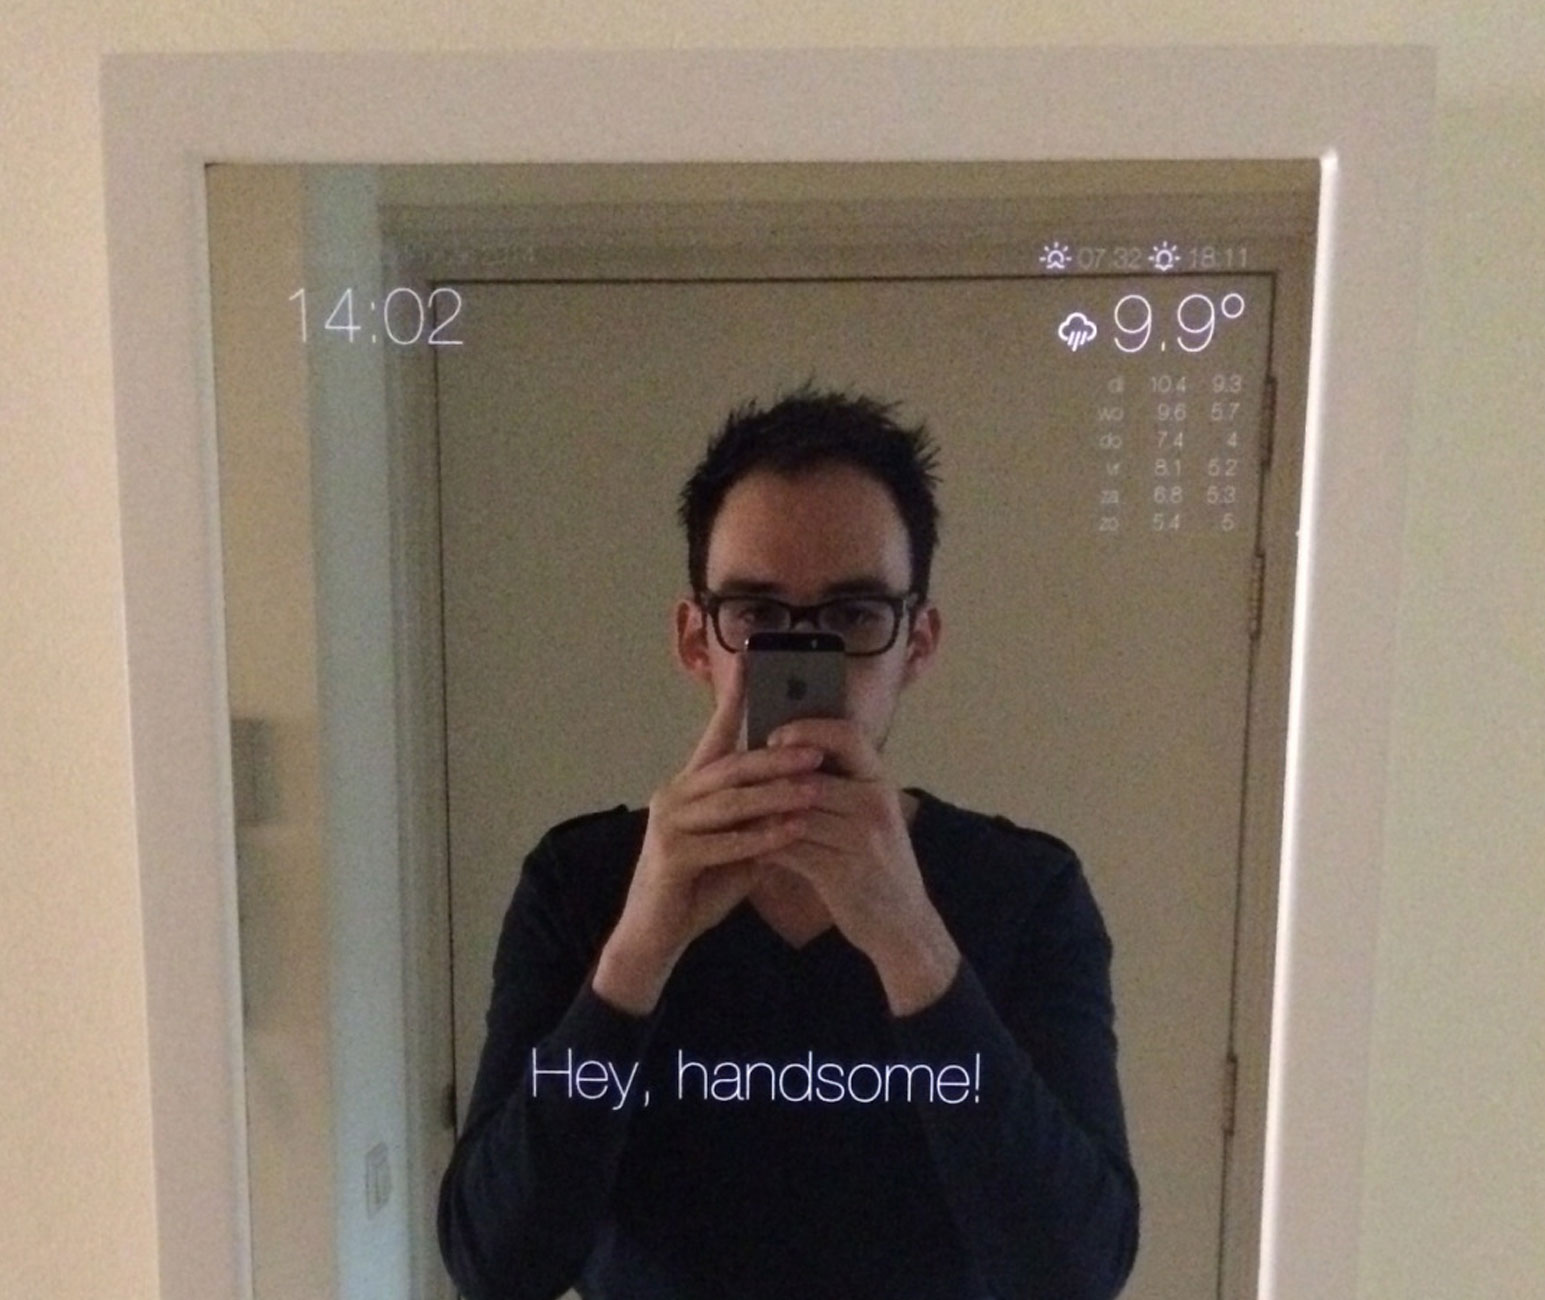
\includegraphics[width=1\textwidth, height=0.6\textheight]{magic_mirror}
    \caption{Magic Mirror by Michael Teeuw}
\end{figure}

\section{Avvio ed Escuzione}
Il Magic Mirror viene avviato tramite riga di comando di una shell: npm start, che va a ricercare
il file javascript principale indicato dal package.json.
All'avvio viene eseguito il codice di Electron, che si occupa della creazione di una nuova finestra, che è l'interfaccia contenente il browser
usato per contenere i DOM e di stampare la relativa pagina HTML, e il codice dell'applicazione, ovvero il corpo principale dello specchio.
Quest'ultima crea e avvia un server per il backend,
il cui compito è di caricare tutte le strtture dati dello specchio:
\begin{itemize}
\item i Moduli, che sono le entità che permettono di creare e configurare applicazioni da agganciare al software principale.
\item i Node Helper, strutture "speciali", opzionali, che servono come supporto esterno ai moduli, per mezzo dei quali si possono interfacciare le api di servizi
esterni al Magic Mirror. Ogni modulo ha il proprio Node Helper con cui può comunicare tramite messaggi in modo simile a come comunicano i moduli tra di loro.
\item un Socket, entità principale che permette lo scambio dei messaggi tra i moduli e i rispettivi Node Helper.
\item un Logger, implementato per tenere i log dell'applicazione e degli evenutali errori. Usato pricipalemnte per il debugging.\\[2\baselineskip]
\end{itemize}
